\UseRawInputEncoding
\documentclass[12pt]{article}
\title{ECE 141 Homework 2}
\usepackage{subcaption}
\author{Lawrence Liu}
\usepackage{graphicx}
\usepackage{amsmath}
\usepackage{placeins}
\newcommand{\Laplace}{\mathscr{L}}
\setlength{\parskip}{\baselineskip}%
\setlength{\parindent}{0pt}%
\usepackage{xcolor}
\usepackage{listings}
\definecolor{backcolour}{rgb}{0.95,0.95,0.92}
\usepackage{amssymb}
\lstdefinestyle{mystyle}{
    backgroundcolor=\color{backcolour}}
\lstset{style=mystyle}

\begin{document}
\maketitle
\section*{Problem 3.21}
\subsection*{(a)}
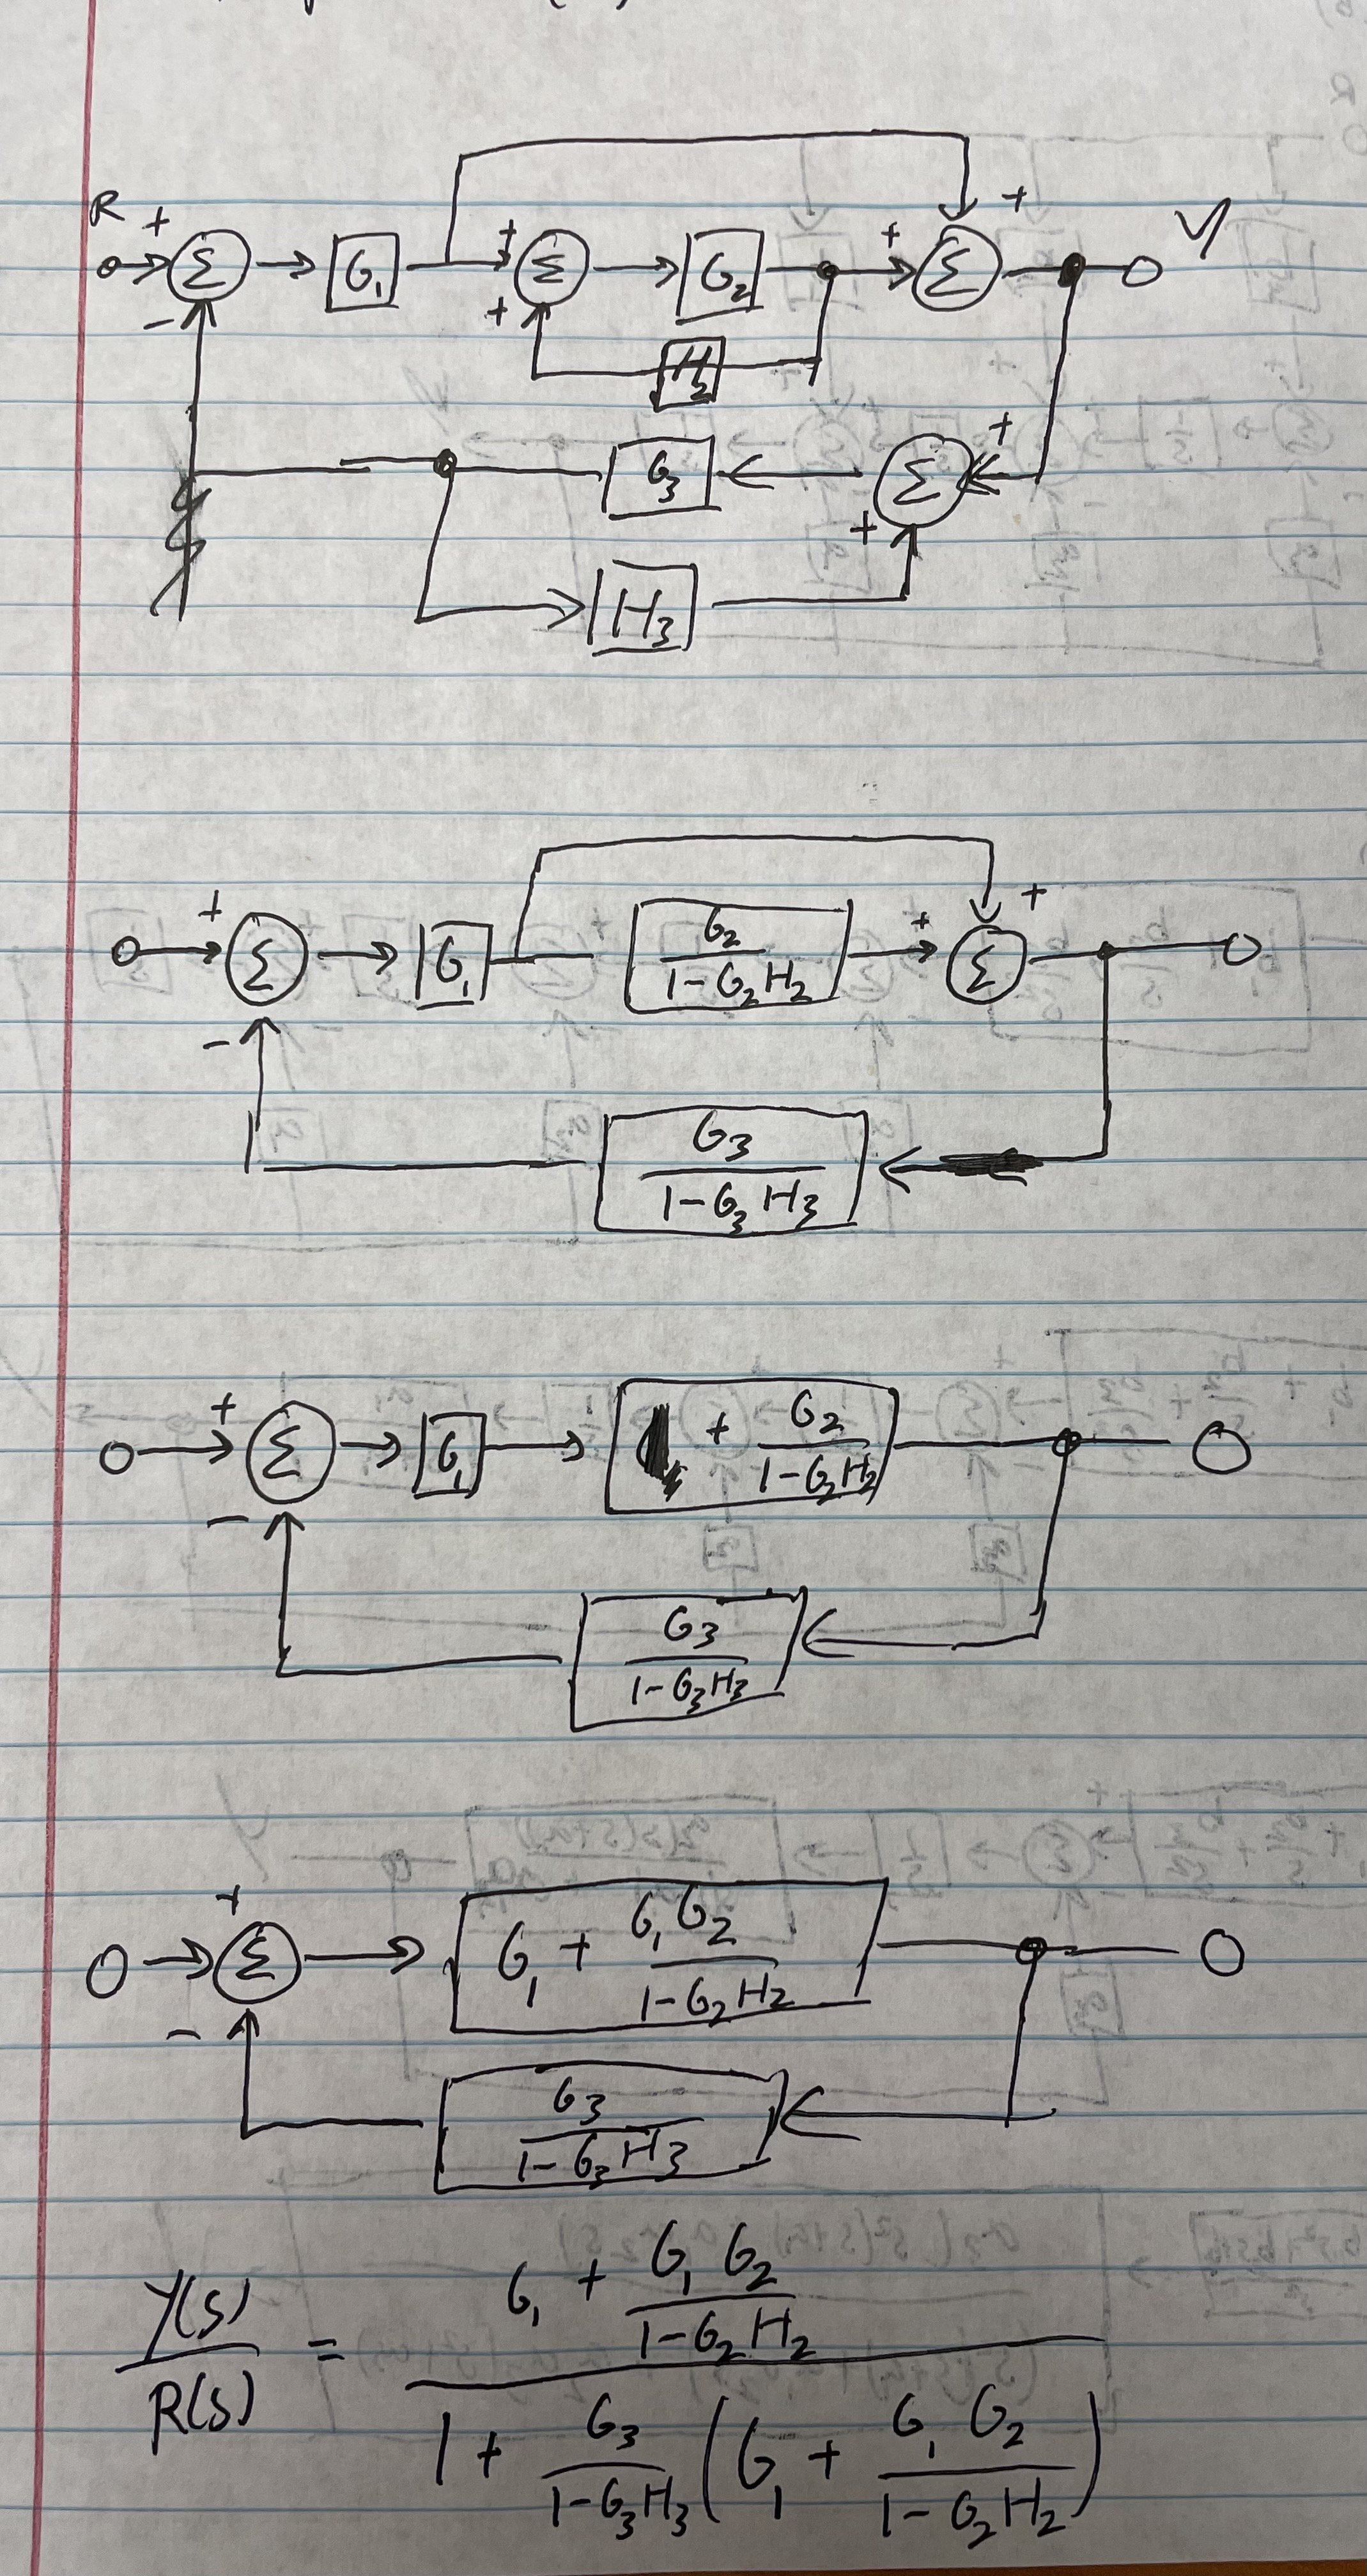
\includegraphics[scale=0.1]{Problem1a.JPG}
\FloatBarrier
$$\frac{Y(s)}{R(s)}=\frac{G_1+\frac{G_1G_2}{1-G_2H_2}}{1+\left(G_1+\frac{G_1G_2}{1-G_2H_2}\right)\frac{G_3}{1-G_3H_3}}$$

\subsection*{(b)}
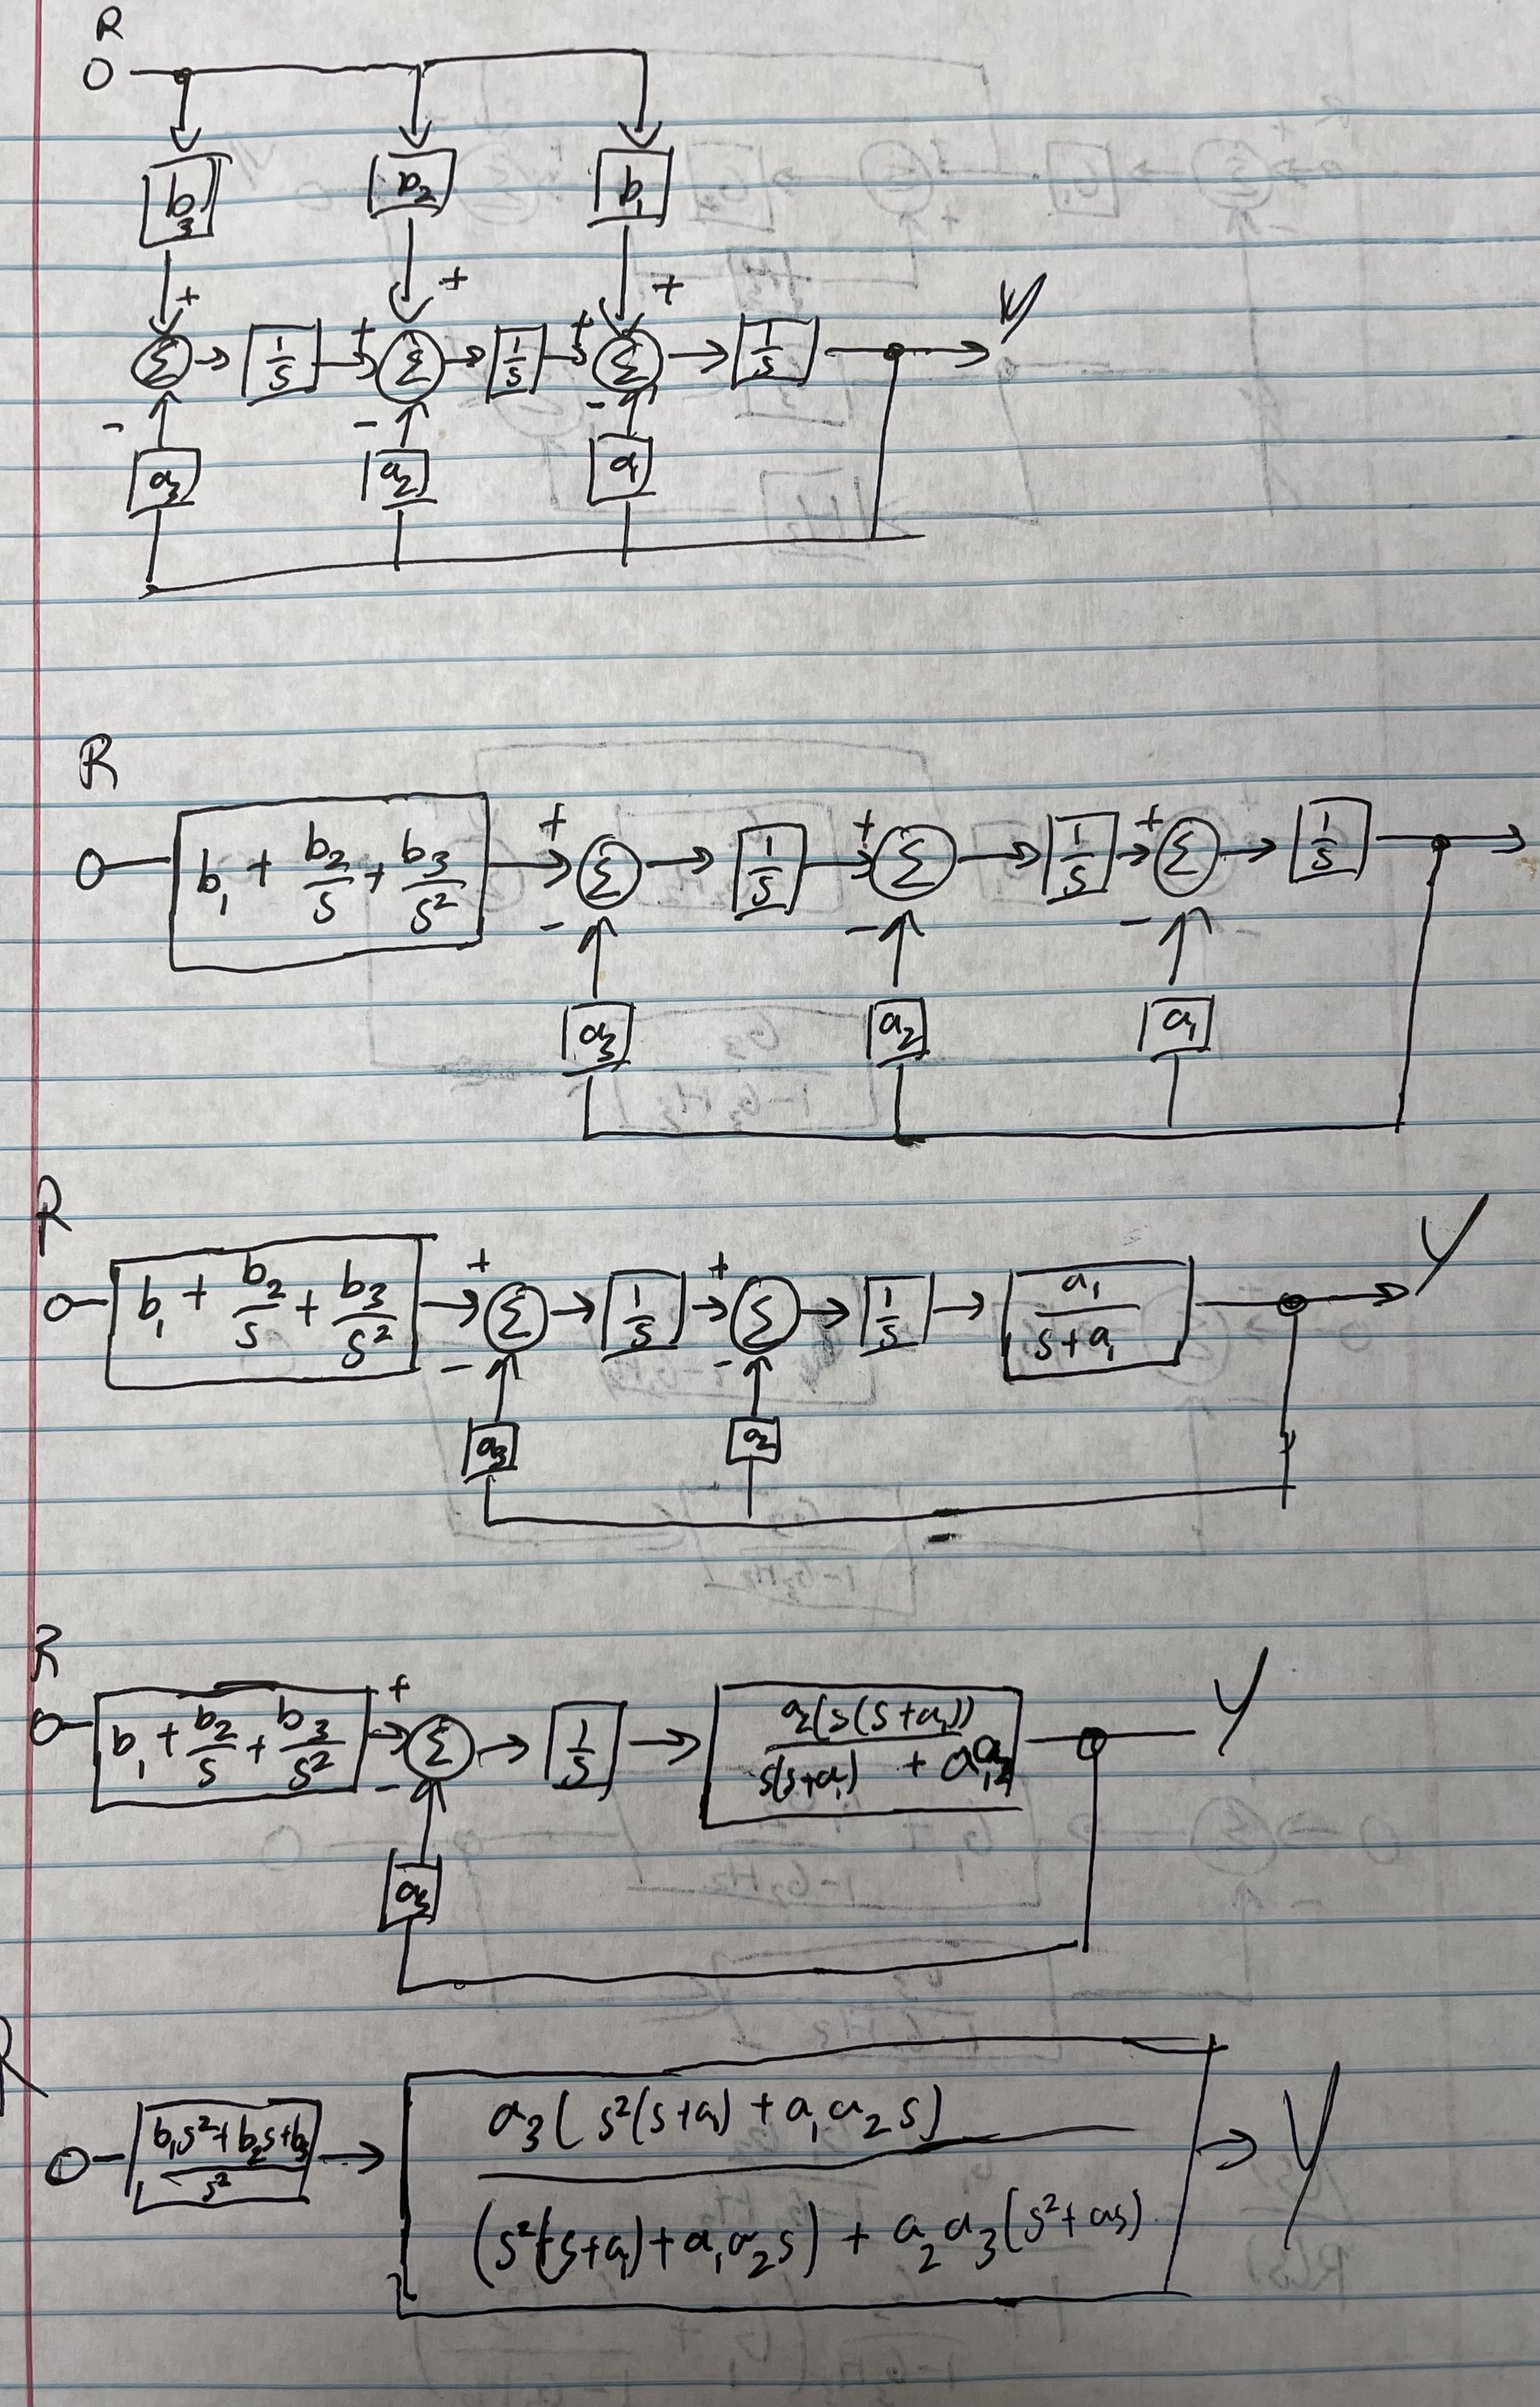
\includegraphics[scale=0.5]{Problem1b.JPG}
\FloatBarrier
$$\frac{Y(s)}{R(s)}=\boxed{\frac{b_1s^2+b_2s+b_3}{s^2}+
\frac{a_3(s^2(s+a_1)+a_1a_2s)}{s^2(s+a_1)+a_1a_2s+a_2a_3(s^2+a_1s)}}$$

\subsection*{(c)}
\includegraphics[scale=0.5,angle=270,origin=c]{Problem1c.JPG}
\FloatBarrier
$$\frac{Y(s)}{R(s)}=\boxed{\frac{b_1s^2+b_2s+b_3}{s^3+a_1s^2+a_2s+a_3}}$$
\subsection*{(d)}
\includegraphics[scale=0.5,angle=270,origin=c]{Problem1d.JPG}
\FloatBarrier
$$\frac{Y(s)}{R(s)}=\boxed{\frac{D(s)+D(s)B(s)H(s)+A(s)B(s)}
{1+B(s)H(s)+G(s)(D(s)+D(s)B(s)H(s)+A(s)B(s))}}$$
\section*{Problem }
\end{document}
